\section{Versuchsaufbau/-durchführung}
Der wesentliche Aufbau eines Sagnac Interfermoeters ist in Abildung \ref{fig:sagnac_interferometer}
dargetsellt.
\begin{figure}
\centering
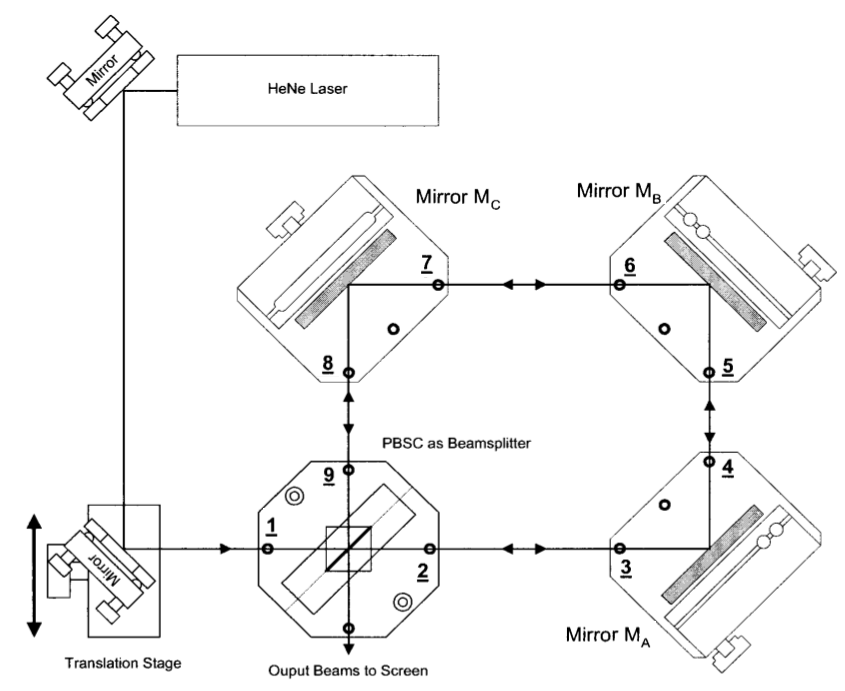
\includegraphics[width=0.7\linewidth]{./content/images/aufbau.png}
\caption{Schmeatischer Aufbau eines Sagnac Interferometers \cite{anleitung64}.}
\label{fig:sagnac_interferometer}
\end{figure}
Als Lichtquelle wird ein $\ce{HeNe}$ Laser mit einer Wellenlänge von
$\lambda\ua{vac}=\SI{632.990}{\nano\meter}$ verwendet. Der Laser wird mittels zweier Spiegel
über einen PBSC in das Interfermoeter eingeleitet. Ausgekoppelt wird das Licht, wie
in Abbildung \ref{fig:sagnac_interferometer} zu erkennen, über die vierte Seite
des Würfels.
Der Ausgangstrahl wird zur Bestimmugn des Brechungsindexes in ein weiteren
PBSC geleitet, der jedoch um $\SI{45}{\degree}$ in der Horizontalen gedreht ist.
Die Drehung des PBSC hat die selbe Auswirkung auf die Polarisation, wie ein Polarisationsfilter mit
einem Filterwinkel von $\SI{45}{\degree}$. Hierdurch wird das zunächst senkrecht
polarisierte Licht (vgl. Abb. \ref{fig:pbsc}) auf die Filterachse projiziert und
ist somit interferenzfähig. Das von dem zweiten PBSC aufgeteilte Licht wird
anschließend auf zwei Photodioden gerichtet.

\subsection{Justage}
Zu Beginn wird der Versuchsaufbau mit einigen Schritten justiert werden.
Erklärt wird die Justage mit den in Abbildung \ref{fig:sagnac_interferometer} verwendeten Bezeichnern.
Nachdem die benötigten Komponenten auf dem optischen Tisch montiert sind,
wird mit Hilfe von zwei Justagehilfen, der Lichtstrahl optimal auf den Spiegel $M_C$
ausgerichtet. Hierbei wird der von $M_A$ kommende Strahl blockiert.
Anschließend werden die Justagehilfe dazu verwende, um den Laserstrahl optimal auf
die Spiegel $M_A$ und $M_B$ auszurichten. Vor dem ersten PCBS wird zusätzlich noch ein Polarisationsfilter
mit einem Filterwinkel von $\SI{45}{\degree}$. Zusätlich werden mit Hilfe der Justagehilfen
und des zweiten Steuersiegels die beiden polarisierten Strahlen horizontal voneinander
getrennt.

Nachdem der Laserstrahl ausgerichtet ist, kann der Laserstrahl an der vierten Seite des PCBS
mit einem Schirm untersucht werden.
Liegen die beiden Strahlen auf dem Schirm nicht aufeinander, wird mit Hilfe der
Feinschrauben der Spiegel $M_A$, $M_B$ und $M_C$ nachjustiert. Wichtig ist das zum
jetzigen Zeitpunkt noch keine Interferenzen beobachtet werden können. Erst nach
dem Einbau eines weiteren Polarisationsfilter (Filterwinkel $\SI{45}{\degree}$)
ist es möglich Interferenzen auf dem Schirm zu erkennen.
Das Interferenzbild soll so eingestellt werden, dass die
"Interferenzfrequenz" null ist, dazu können die Feinschrauben der Spiegel
$M_A$ und $M_C$ verwendet werden.

Wurde die "Interferenzfrequenz" minimiert, wird der zweite Polarisationsfilter wieder
entfernt und stattdessen der um $\SI{45}{\degree}$ geneigte PBSC mit den Photodioden
montiert. Bevor nun die Brechungsindices vo Luft und Glas bestimmt werden, wird eine
Kontrastbestimmung durchgeführt. Hierzu mehr im nächsten Kapitel.

\subsection{Kontrastbestimmung}
Der Kontrast des Interferometers ist ein Maß für das Auflösungsvermögen und wird
wie folgt definiert
\begin{equation}
  \label{eq:kontrast}
  K = \frac{I\ua{max} - I\ua{min}}{I\ua{max}+I\ua{min}}.
\end{equation}
Für die Bestimmung der Intensitäten $I\ua{max}$ und $I\ua{min}$ wird der zweite
PBSC und die Glasprobe benötigt.
Die Glasrpo
Hierzu wird eine Glaseprobe in den Strahlengang montiert. Die Glasprobe
besteht aus zwei Gläsern die jeweils zu einem der horizontal seperierten Strahlen
im Interfermoter einen Winkel von $\SI{10}{\degree}$ steht. Durch die Gläser soll
ein Gangunterschied bzw. eine Phasendifferenz zwischen den beiden Strahl erzeugt werden.
Hierzu wird kann die Probe um $\SI{10}{\degree}$ gedreht werden. Zu beachten ist, dass
bei einer beispielweisen Drehung der Probe um $\SI{1}{\degree}$, ein Glas
einen Winkel von $\SI{9}{\degree}$ und das Andere von $\SI{11}{\degree}$ zu den jeweiligen
Strahlen besitzen. Die Intensität wird nun mit Hilfe einer Photodiode und einem Oszilloskop
gemessen. Die Messungen erfolgen bei verschiedenen Filterwinkeln des Polarisationsfilters.
